% ============================================================================
% IRT-LSEM Manuscript — HNUE Journal of Science (mẫu bài tiếng Việt)
%
% Build:   make pdf       (latexmk -xelatex)
% Spec:    "Mau bao cao Tieng Viet.docx" của Tạp chí — xem style/hnue.sty
% ============================================================================
\documentclass[11pt,twoside]{article}

% --- Font: Times New Roman (XeLaTeX + fontspec), toán kiểu Times ------------
\usepackage{mathptmx}
\usepackage[no-math]{fontspec}
\setmainfont{Times New Roman}
\usepackage{polyglossia}
\setdefaultlanguage{vietnamese}
\setotherlanguage{english}

% --- Page geometry: 19x27 cm, lề đối xứng chẵn/lẻ ----------------------------
% Top 2,5 / Bottom 2 / Inside 3 / Outside 1 cm; header/footer cách mép 1,5 cm.
\usepackage{geometry}
\geometry{paperwidth=19cm, paperheight=27cm, twoside,
          top=2.5cm, bottom=2cm, inner=3cm, outer=1cm,
          headheight=0.5cm, headsep=0.5cm, footskip=0.5cm}

% --- Body text spec: single, first line 0,75 cm, before/after 2 pt ----------
\usepackage{setspace}\singlespacing
\usepackage{indentfirst}
\setlength{\parindent}{0.75cm}
\setlength{\parskip}{2pt}
\renewcommand{\arraystretch}{1.0}
\setlength{\tabcolsep}{4pt}
\setlength{\textfloatsep}{6pt}
\setlength{\intextsep}{4pt}
\setlength{\floatsep}{6pt}

% --- Math + tables + figures + links ----------------------------------------
\usepackage{amsmath,amssymb}
\usepackage{booktabs,array}
\usepackage{float}                       % [H] force inline figures
\usepackage{graphicx}
\graphicspath{{figures/}}
\usepackage{multicol}
\usepackage{tikz}
\usetikzlibrary{positioning, arrows.meta, shapes.geometric, fit, calc}
\usepackage{cite}                        % numeric [1], [2]-[5] auto-collapse
\usepackage[breaklinks=true,hidelinks]{hyperref}
\usepackage{xurl}
\urlstyle{same}

% --- Page numbering: Different odd and even, Different first page ----------
\usepackage{fancyhdr}
\pagestyle{fancy}\fancyhf{}
\fancyfoot[LE,RO]{\thepage}
\renewcommand{\headrulewidth}{0pt}
\renewcommand{\footrulewidth}{0pt}

% --- HNUE-specific macros + heading specs -----------------------------------
\usepackage{style/hnue}

% ----------------------------------------------------------------------------
\begin{document}

\thispagestyle{empty}

% ============================================================================
% Trang đầu theo "Mau bao cao Tieng Viet.docx" của Tạp chí:
%   - Tên bài: IN HOA, đậm, 11pt, căn giữa.
%   - Tác giả: chữ thường viết hoa đầu, 12pt; đơn vị: in nghiêng, 11pt.
%   - Tóm tắt + từ khóa: 10pt, 3--5 câu, 3--5 từ khóa.
%   - Ngày nhận bài + tác giả liên hệ: chú thích cuối trang 1 (không dấu).
%   - Phần tiếng Anh (ABSTRACT) đặt cuối bài: sections/07_abstract_en.tex.
% ============================================================================

\begin{center}
{\fontsize{11}{13}\bfseries\selectfont
ƯỚC LƯỢNG NĂNG LỰC ĐỘNG CỦA HỌC SINH DỰA TRÊN LÝ THUYẾT ĐÁP ỨNG CÂU HỎI (IRT) VÀ MÔ HÌNH PHƯƠNG TRÌNH CẤU TRÚC DỌC (LSEM)}
\end{center}

\vspace{4pt}

\begin{center}
{\fontsize{12}{14}\selectfont
Nguyễn Tiến Đạt\textsuperscript{1}}
\end{center}

\begin{center}
{\fontsize{11}{13}\itshape\selectfont
\textsuperscript{1}Khoa Công nghệ Thông tin, Trường Toán học và Công nghệ thông tin,\\
Trường Đại học Sư phạm Hà Nội, Hà Nội, Việt Nam}
\end{center}

% Chú thích cuối trang 1: ngày tháng do Toà soạn điền.
\begingroup
\renewcommand{\thefootnote}{}
\renewcommand{\footnoterule}{\vspace*{-3pt}\noindent\rule{0.3\linewidth}{0.4pt}\vspace*{2.6pt}}
\footnotetext{\hspace*{-1.8em}\fontsize{10}{12}\selectfont
Ngày nhận bài: \ldots/\ldots/\ldots. Ngày sửa bài: \ldots/\ldots/\ldots. Ngày nhận đăng: \ldots/\ldots/\ldots.\\
Tác giả liên hệ: Nguyễn Tiến Đạt. Địa chỉ e-mail: \href{mailto:mas835151465@hnue.edu.vn}{mas835151465@hnue.edu.vn}; \href{mailto:dat.dtnntd@gmail.com}{dat.dtnntd@gmail.com}}
\endgroup

\vspace{4pt}

{\fontsize{10}{12}\selectfont
\setlength{\leftskip}{1cm}\setlength{\rightskip}{1cm}
\noindent\textbf{Tóm tắt.} Các hệ thống Lý thuyết Đáp ứng câu hỏi (IRT) triển khai quy mô lớn, kể cả nền tảng OLM của Việt Nam, thường giả định năng lực học sinh \(\theta\) là tĩnh, trong khi dữ liệu học trực tuyến dày đặc theo thời gian lại mâu thuẫn với giả định này. Bài báo xây dựng và kiểm chứng khung tích hợp IRT--LSEM nhằm ước lượng năng lực động \(\theta_{it}\) trên dữ liệu Toán THPT từ OLM gồm 24{.}213 học sinh và 122{.}957 lượt đánh giá ở các khối 10--12. Khung gồm tầng đo lường 1PL (ước lượng EAP) kết hợp bốn biến thể cấu trúc dọc (LGCM, LCSM, mô hình đa cấp, CT-DSEM) và bộ lọc Kalman sử dụng sai số chuẩn EAP làm phương sai quan sát biến thiên theo thời gian. Mô hình động vượt mô hình tĩnh cơ sở với \(\Delta\)AIC = 82--167 (LRT \(p \le 10^{-19}\)); LCSM phát hiện cơ chế đuổi kịp ở khối 10 (\(\beta = -0{,}069\), khoảng tin cậy không chứa 0) chuyển sang trạng thái ổn định (\(\beta \approx 0\)) ở khối 12; bộ lọc Kalman giảm 32--41\% phương sai sai số đo lường mà không cần tăng số câu hỏi. Khung phương pháp đề xuất đặt nền tảng cho hướng phát triển ước lượng năng lực thời gian thực thông qua Suy diễn Biến phân trực tuyến.\par
\noindent\textbf{\textit{Từ khóa:}} lý thuyết đáp ứng câu hỏi, mô hình phương trình cấu trúc dọc, bộ lọc Kalman, ước lượng năng lực động, khai phá dữ liệu giáo dục.
\par}

\vspace{6pt}


% ============================================================================
% §1 Giới thiệu — bám đề cương NCKH (docs/nckh/de_cuong), văn phong tiếng Việt
% học thuật, hạn chế trộn lẫn thuật ngữ tiếng Anh không cần thiết.
% ============================================================================

\section{Mở đầu}
\label{sec:intro}

Cùng với quá trình chuyển đổi số diễn ra mạnh mẽ trong lĩnh vực giáo dục, việc đo lường và theo dõi năng lực học sinh trở thành một yêu cầu then chốt đối với chất lượng dạy và học. Tuy nhiên, thực tiễn hiện nay cho thấy việc đánh giá năng lực học sinh vẫn chủ yếu dựa trên các bài kiểm tra tại từng thời điểm cố định, không phản ánh được bản chất động của quá trình học tập. Trong lý thuyết đo lường giáo dục, có thể phân biệt hai quan điểm về năng lực: \emph{năng lực tĩnh} giả định \(\theta_i\) là hằng số đối với từng học sinh --- giả định cốt lõi của Lý thuyết Đáp ứng câu hỏi (IRT) truyền thống \cite{lord1980,hambleton1991}; và \emph{năng lực động} \(\theta_{it}\) thay đổi theo thời gian \(t\), phản ánh quá trình học tập liên tục \cite{kim2023,pengwei2022}. Khi quá trình học tập diễn ra song song với quá trình đánh giá, giả định năng lực tĩnh trở nên không còn phù hợp.

IRT đã được chứng minh là phương pháp hiệu quả để đo lường năng lực tiềm ẩn thông qua mô hình hoá xác suất trả lời đúng \cite{chalmers2012}, với ưu điểm là tách được tham số năng lực của người học khỏi tham số độ khó của đề thi. Tuy nhiên, hầu hết các mô hình IRT truyền thống đều dựa trên giả định năng lực tĩnh \cite{lord1980}. Hệ thống học trực tuyến OLM (\url{https://olm.vn}) tại Việt Nam hiện sử dụng mô hình Rasch 1PL --- chỉ ước lượng một giá trị \(\theta\) duy nhất cho mỗi học sinh tại một thời điểm và chưa có cơ chế theo dõi sự thay đổi năng lực qua nhiều kỳ thi. Trong khi đó, các mô hình phương trình cấu trúc dọc (Longitudinal Structural Equation Models, LSEM) cho phép theo dõi sự thay đổi của biến tiềm ẩn theo thời gian \cite{mcardle2009}. Khi kết hợp IRT với LSEM, có thể xây dựng được mô hình đánh giá năng lực động phản ánh sát hơn thực tế học tập; tuy vậy, việc khai thác hiệu quả nguồn dữ liệu lớn từ các hệ thống học trực tuyến để phân tích quỹ đạo năng lực vẫn là một thách thức chưa được giải quyết thoả đáng.

\textbf{Nghiên cứu ngoài nước:} Hướng nghiên cứu IRT trực tuyến (Online IRT, OIRT) cập nhật ước lượng năng lực liên tục mỗi khi có dữ liệu mới, thông qua Suy diễn Biến phân (\emph{Variational Inference}) \cite{pengwei2022}. Mô hình VTIRT (Variational Temporal IRT) đã chứng minh khả năng theo dõi năng lực động trên chín bộ dữ liệu thực tế, với tốc độ nhanh hơn MCMC nhiều bậc độ lớn \cite{kim2023}. Các mô hình DSEM được phát triển để xử lý dữ liệu dọc, cho phép phân tích sự biến đổi năng lực ở cả cấp cá nhân lẫn cấp nhóm \cite{asparouhov2018}; khi khoảng cách giữa các đợt đánh giá không đồng đều, biến thể thời gian liên tục CT-DSEM được sử dụng để bảo toàn tính xác định của mô hình \cite{driver2017}. Mô hình RI-CLPM được dùng để phân tách hiệu ứng đặc trưng ổn định của cá nhân (\emph{trait-like}) khỏi biến động trong nội bộ cá nhân (\emph{within-person}) \cite{hamaker2015}. Trên thực tế triển khai, Duolingo sử dụng phương pháp hồi quy bán chu kỳ (\emph{Half-Life Regression}) \cite{settles2016}; Khan Academy dùng phương pháp theo dõi tri thức Bayes (\emph{Bayesian Knowledge Tracing}); IXL sử dụng đánh giá chẩn đoán dựa trên IRT --- tuy nhiên các hệ thống này chủ yếu theo dõi năng lực trong phạm vi một phiên học, chưa kết hợp IRT với LSEM để phân tích quỹ đạo tăng trưởng qua nhiều kỳ thi \cite{cambium2020}.

\textbf{Nghiên cứu trong nước:} Tại Việt Nam, ứng dụng IRT chủ yếu dừng lại ở việc đánh giá độ khó đề thi và ước lượng năng lực tĩnh \cite{nguyen_tan}. Các nghiên cứu đăng trên Tạp chí Khoa học Trường Đại học Sư phạm Hà Nội cũng dùng IRT để phân tích và thẩm định đề kiểm tra tại một thời điểm, như phân tích phần Đọc hiểu của đề thi thử VSTEP bậc 3--5 \cite{dao2025vstep}; kiểm tra đánh giá trực tuyến ở trường phổ thông mới được khảo sát dưới góc độ tác động sư phạm \cite{ngo2025ofa}, chưa khai thác chuỗi dữ liệu đáp ứng để theo dõi năng lực theo thời gian. Hệ thống OLM đã tích luỹ một lượng dữ liệu học tập rất lớn nhưng hiện chỉ sử dụng Rasch 1PL cho ước lượng tĩnh. Việc kết hợp IRT với các mô hình cấu trúc dọc và ước lượng năng lực động trên dữ liệu quy mô lớn vẫn là một khoảng trống nghiên cứu đáng kể, đặc biệt trong bối cảnh dữ liệu giáo dục Việt Nam.

\textbf{Khoảng trống và phát biểu bài toán:} Từ phân tích trên, ba khoảng trống cụ thể được nhận diện: (i) thiếu các mô hình tích hợp IRT--LSEM phục vụ đo lường năng lực động trong bối cảnh dữ liệu giáo dục Việt Nam; (ii) chưa có thuật toán ước lượng năng lực có khả năng cập nhật đệ quy sau mỗi đợt đánh giá phù hợp với dữ liệu lớn từ hệ thống học trực tuyến; (iii) chưa khai thác dữ liệu thực tế để phân tích quỹ đạo phát triển năng lực và hỗ trợ ra quyết định sư phạm. Bài toán nghiên cứu được phát biểu như sau: \emph{cho ma trận đáp ứng \(Y_{ijt} \in \{0,1\}\) của \(N\) học sinh, \(J_t\) câu hỏi qua \(T\) đợt đánh giá, hãy đồng thời ước lượng tham số câu hỏi \(b_j\), năng lực động \(\theta_{i1}, \theta_{i2}, \dots, \theta_{iT}\) tại mỗi thời điểm và mô hình hoá quỹ đạo thay đổi của chuỗi năng lực này.} Bài báo xây dựng mô hình không gian-trạng thái làm nền cho cơ chế cập nhật đệ quy; bản hiện thực trực tuyến được để lại cho nghiên cứu tiếp theo.

\textbf{Đóng góp của bài báo:} (1) Đề xuất một khung tích hợp IRT--LSEM tổng quát kèm quy trình phân tích bảy bước có thể tái lập đầy đủ, bao gồm tầng đo lường IRT 1PL với ước lượng Bayes (EAP) và bốn biến thể cấu trúc (LGCM, LCSM, mô hình tăng trưởng đa cấp, CT-DSEM thời gian liên tục cho khoảng cách thời gian không đồng đều). (2) Cung cấp bằng chứng định lượng từ \(N = 24{.}213\) học sinh THPT Việt Nam cho thấy mô hình động vượt mô hình tĩnh cơ sở. (3) Bộ làm trơn Kalman (hồi cứu) lấy sai số chuẩn EAP làm phương sai quan sát biến thiên theo thời gian, giảm phương sai sai số đo lường \emph{mà không cần thêm câu hỏi}. (4) Hai ứng dụng dẫn xuất --- cảnh báo sớm học sinh có dấu hiệu giảm năng lực và gợi ý câu hỏi tối đa hoá thông tin --- được minh hoạ trên quỹ đạo thực tế.

% ============================================================================
% §2 Nội dung nghiên cứu (Research Content) — parent file
% Includes 4 subfiles 03a-03d.
% ============================================================================

\section{Nội dung nghiên cứu}
\label{sec:content}

% ============================================================================
% §2.1 Phương pháp — IRT, LSEM, CT-DSEM, Kalman, ứng dụng. Văn phong tiếng Việt
% học thuật, giảm code-switching không cần thiết.
% ============================================================================

\subsection{Phương pháp}
\label{sec:methods}

Khung phương pháp gồm hai tầng (Hình~\ref{fig:pipeline}): tầng \emph{đo lường} sử dụng IRT để chuyển dữ liệu đáp ứng nhị phân thành ước lượng năng lực; tầng \emph{cấu trúc} sử dụng LSEM để phân tích quỹ đạo của năng lực theo thời gian. Bộ lọc Kalman cục bộ làm trơn các ước lượng năng lực ở tầng đo lường, đồng thời tận dụng sai số đo \(\seit\) làm phương sai quan sát biến thiên theo thời gian.

\subsubsection{Tầng đo lường: IRT 1PL và chấm điểm EAP}

Mô hình Rasch một tham số (1PL) xác định xác suất trả lời đúng câu \(j\) của học sinh \(i\):
\begin{equation}
P(Y_{ij}=1 \mid \theta_i, b_j) = \sigma(\theta_i - b_j), \quad \sigma(x) = (1+e^{-x})^{-1}.
\label{eq:1pl}
\end{equation}
Tham số độ khó \(b_j\) được ước lượng bằng phương pháp hợp lý cực đại biên (\emph{Maximum Marginal Likelihood}) thông qua gói \texttt{mirt} \cite{chalmers2012}. Năng lực \(\hat{\theta}_{it}\) tại mỗi đợt đánh giá được ước lượng bằng phương pháp kỳ vọng hậu nghiệm (\emph{Expected A Posteriori}, EAP) với phân phối tiên nghiệm \(\Norm(0,1)\), kèm sai số chuẩn \(\seit = \sqrt{\Var(\theta\mid\mathbf{y}_{it})}\). Mô hình 1PL được chọn thay cho 2PL/3PL vì lý do thực nghiệm và lý thuyết. Về thực nghiệm: khi ước lượng 2PL trên bộ dữ liệu hiện có, có 2--6\% câu hỏi cho tham số phân biệt (\emph{discrimination}) thoái hoá --- tức $\hat a_j \to 0$ (câu không phân biệt được học sinh) hoặc $\hat a_j < 0$ (câu phân biệt ngược, học sinh giỏi trả lời sai nhiều hơn), gây nhiễu cho ước lượng năng lực; trong khi đó, 1PL ổn định trên toàn ngân hàng câu hỏi. Về lý thuyết: 1PL (Rasch) giả định mọi câu phân biệt ở cùng mức, phù hợp với mục tiêu so sánh độ khó tuyệt đối giữa các câu và tạo thang đo \(\theta\) có tính nhất quán nội tại (\emph{specific objectivity}) \cite{lord1980}.

\subsubsection{Tầng cấu trúc: bốn biến thể LSEM}

\textit{Mô hình tăng trưởng tiềm ẩn (LGCM)} \cite{mcardle2009} mô hình hoá đồng thời điểm xuất phát và tốc độ tăng trưởng của cá nhân trên bốn đợt đầu của mỗi học sinh (\(t = 0,\dots,3\); FIML cho đợt thiếu), LCSM dùng cùng cửa sổ:
\begin{equation}
\hat{\theta}_{it} = \alpha_i + s_i\,t + \varepsilon_{it}, \quad (\alpha_i, s_i)^\top \sim \Norm\big((\alpha, s)^\top,\ \Sigma\big).
\label{eq:lgcm}
\end{equation}
\textit{Mô hình điểm thay đổi tiềm ẩn (LCSM)} bổ sung hệ số ghép cặp \(\beta\) giữa các thời điểm liên tiếp:
\begin{equation}
\Delta \theta_{it} = \alpha + \beta\,\theta_{i,t-1} + \zeta_{it}.
\label{eq:lcsm}
\end{equation}
\(\beta < 0\) thể hiện cơ chế đuổi kịp (học sinh yếu tăng nhanh hơn học sinh khá); \(\beta \approx 0\) biểu thị trạng thái ổn định. \textit{Mô hình tăng trưởng đa cấp (lmer)} dùng REML trên \emph{toàn bộ} chuỗi đợt của mỗi học sinh và được dùng để đối chiếu chiều của độ dốc. \textit{Mô hình CT-DSEM} (Ornstein--Uhlenbeck \cite{driver2017,asparouhov2018}) chỉ được áp dụng cho khối~12 vì hai lý do: (i) CT-DSEM đòi hỏi mỗi cá nhân có đủ nhiều đợt quan sát (chuẩn vàng \(T_i \ge 10\text{--}15\)) để ước lượng các tham số dynamics ở cấp cá nhân được tin cậy --- chỉ khối 12 có một tập con đủ lớn \(N = 460\) học sinh thoả \(T_i \ge 15\) (xem Bảng~\ref{tab:samples}: \(T_{\max} = 37\) ở khối 12 so với 17 và 22 ở khối 10, 11); (ii) khoảng cách thời gian \(\Delta t\) giữa các đợt đánh giá ở khối 12 trải năm bậc độ lớn (từ vài phút đến vài tháng), khiến mô hình thời gian rời rạc (DSEM) không còn phù hợp và bắt buộc phải dùng biến thể thời gian liên tục:
\begin{equation}
d\theta_{it} = (\varphi\,\theta_{it} + \kappa)\,dt + \sigma\,dW_t,
\label{eq:ctdsem}
\end{equation}
trong đó \(\varphi < 0\) biểu thị động lực quay về cân bằng, \(\kappa\) là hằng số trôi; điểm cân bằng dài hạn \(\theta_{\mathrm{eq}} = -\kappa/\varphi\) và bán chu kỳ \(\ln 2 / |\varphi|\) đặc trưng cho tốc độ tiến về cân bằng. Mô hình RI-CLPM \cite{hamaker2015} không được sử dụng do dữ liệu hiện tại chỉ có một biến tiềm ẩn (năng lực Toán \(\theta\)); trong trường hợp đơn biến, RI-CLPM trở nên thừa tham số và quy về một mô hình AR(1) ngẫu nhiên, không cung cấp thêm thông tin so với CT-DSEM. Khoảng tin cậy 95\% cho các hệ số LGCM/LCSM được tính bằng \emph{bias-corrected bootstrap} với 1{.}000 mẫu (lavaan); khoảng tin cậy cho hệ số đa cấp tính theo Wald từ ma trận thông tin Fisher (lme4); khoảng tin cậy cho CT-DSEM tính theo Hessian xấp xỉ tại điểm MAP (ctsem).

\subsubsection{Bộ lọc Kalman cục bộ với phương sai quan sát biến thiên}

Đối với mỗi học sinh \(i\), mô hình không gian-trạng thái tuyến tính được thiết lập như sau: phương trình trạng thái \(\theta_{it} = \theta_{i,t-1} + u_{it}\) với nhiễu trạng thái \(u_{it} \sim \Norm(0,\, q_g)\), và phương trình quan sát \(\hat{\theta}_{it} = \theta_{it} + \varepsilon_{it}\) với \(\Var(\varepsilon_{it}) = \seit^{2}\). Điểm mới so với cách áp dụng Kalman thông thường là phương sai quan sát \(H_t = \seit^2\) được lấy trực tiếp từ Phương trình~\eqref{eq:1pl} thông qua thuật toán EAP, biến thiên theo số câu hỏi mà mỗi học sinh hoàn thành trong từng đợt. Phương sai trạng thái \(q_g\) được ước lượng chung ở cấp khối bằng phương pháp khớp moment (\emph{moment matching}): \(\hat q_g = \overline{\Delta\hat{\theta}^2} - \overline{\seit^2 + \mathrm{SE}_{i,t-1}^2}\). Thuật toán làm trơn được thực hiện bằng gói \texttt{KFAS::KFS} \cite{helske2017}, ổn định ngay cả trên chuỗi quan sát ngắn (\(T \ge 2\)). Mở rộng sang quan sát phi tuyến (1PL/2PL) thông qua Suy diễn Biến phân đã được phác thảo trong tài liệu thiết kế kèm theo nhưng chưa có mã chạy thực tế.

\subsubsection{Ứng dụng: cảnh báo sớm và gợi ý câu hỏi}

\textit{Cảnh báo sớm học sinh có dấu hiệu giảm năng lực (B7a):} Một học sinh được đánh dấu nếu thoả mãn ít nhất một trong hai tiêu chí: (a) tốc độ tăng trưởng \(s_i < Q_{10}(s)\) --- thuộc nhóm 10\% thấp nhất trong khối; (b) \(\min_t \Delta\theta_{i,t}^{\,\mathrm{smooth}} < -1\) logit --- xuất hiện một bước giảm đột ngột vượt mức 2,5 lần sai số chuẩn sau làm trơn. Tốc độ tăng trưởng cho tiêu chí (a) được trích từ thành phần ngẫu nhiên (\texttt{ranef}) của mô hình lmer, không phải từ hồi quy OLS riêng cho từng cá nhân; tín hiệu giảm dùng cho tiêu chí (b) lấy từ quỹ đạo đã làm trơn bằng Kalman thay vì từ \(\hat\theta\) thô, nhằm hạn chế tỷ lệ dương tính giả.

\textit{Gợi ý câu hỏi tối đa hoá thông tin (B7b):} Trong mô hình 1PL, hàm thông tin Fisher \(I(\theta,b) = \sigma(\theta-b)(1-\sigma(\theta-b))\) đạt cực đại tại \(b = \theta\). Bộ gợi ý chọn \(k\) câu có \(|b - \hat{\theta}_{i,T}| < \delta\) (mặc định \(\delta = 0{,}5\)) từ ngân hàng câu hỏi của khối tương ứng.

% ============================================================================
% §2.2 Dữ liệu và pipeline. Mô tả nguồn dữ liệu chi tiết hơn + pipeline TikZ
% cân đối lại (vertical hai hàng để cân nhánh đo lường / cấu trúc / ứng dụng).
% ============================================================================

\subsection{Dữ liệu và quy trình xử lý}
\label{sec:data}

\subsubsection{Nguồn dữ liệu}

Dữ liệu sử dụng là nhật ký đáp ứng của hệ thống học trực tuyến \textbf{OLM} (\url{https://olm.vn}) --- một nền tảng giáo dục lớn ở Việt Nam phục vụ khoảng \(>\)\,1 triệu học sinh phổ thông. Nghiên cứu trích nhật ký môn \textbf{Toán} của ba khối THPT (khối 10, khối 11, khối 12) trong năm học \textbf{2024--2025} (tháng 9/2024 đến tháng 5/2025). Mỗi bản ghi ứng với một lượt làm bài của học sinh \emph{i} trên câu hỏi \emph{j} tại thời điểm \emph{t}, được mã hoá thành biến nhị phân \(Y_{ijt} \in \{0,1\}\) (đúng/sai).

Nhật ký bao gồm hai loại đánh giá: (i) \emph{bài luyện tập} do học sinh chủ động làm và không tính điểm; (ii) \emph{bài kiểm tra} do giáo viên giao và chấm điểm. Hai loại đánh giá này dùng chung một ngân hàng câu hỏi, do đó tham số độ khó \(b_j\) có thể được hiệu chuẩn đồng thời trên cả hai nguồn. Không có thông tin lớp học vật lý (\texttt{class\_id}), giáo viên hay trường trong lược đồ dữ liệu (\emph{schema}) OLM Toán hiện hành; do đó nghiên cứu này thực hiện phân tích ở cấp khối lớp, chưa thể phân tích ở cấp lớp hay cấp trường.

\textbf{Tiêu chí lọc:} (a) Loại học sinh có \(T_i = 1\) (không có đủ đợt để mô hình hoá quỹ đạo); (b) loại các đợt có số câu trả lời \(n_{\mathrm{items},it} < 5\) (nhiễu đo lường lớn); (c) loại câu hỏi xuất hiện \(< 30\) lần (không đủ ước lượng \(b_j\)). Sau lọc, tập phân tích còn \textbf{24{.}213 học sinh} và \textbf{122{.}957 lượt đánh giá} (Bảng~\ref{tab:samples}). Trung vị số đợt mỗi học sinh là 4--5; chỉ khối~12 có một tập con đáng kể đạt \(T_i \ge 15\) (Hình~\ref{fig:Tdt} trái), trong khi khoảng cách thời gian \(\Delta t\) giữa hai đợt liên tiếp trải năm bậc độ lớn --- từ vài phút đến vài tháng (Hình~\ref{fig:Tdt} phải) --- là đặc tính đòi hỏi mô hình động ở thời gian liên tục (CT-DSEM) thay vì DSEM rời rạc.

\begin{figure}[H]
\centering
\begin{minipage}[c]{0.50\linewidth}
  \centering\small
  \captionof{table}{Quy mô mẫu sau lọc (OLM Toán, năm học 2024--2025).}
  \label{tab:samples}
  \resizebox{\linewidth}{!}{%
  \begin{tabular}{lrrr}
  \toprule
  \textbf{Đại lượng} & \textbf{K10} & \textbf{K11} & \textbf{K12} \\
  \midrule
  Số học sinh ($N$)              & 6{.}407 & 7{.}002 & 10{.}804 \\
  Số lượt ($\sum_i T_i$)          & 32{.}191 & 29{.}959 & 60{.}807 \\
  Số câu hỏi (ngân hàng)         & 3{.}277 & 3{.}473 & 8{.}236 \\
  $T_{\mathrm{median}}$           & 4 & 4 & 5 \\
  $T_{\max}$                       & 17 & 22 & 37 \\
  \bottomrule
  \end{tabular}%
  }
\end{minipage}\hfill
\begin{minipage}[c]{0.46\linewidth}
  \centering
  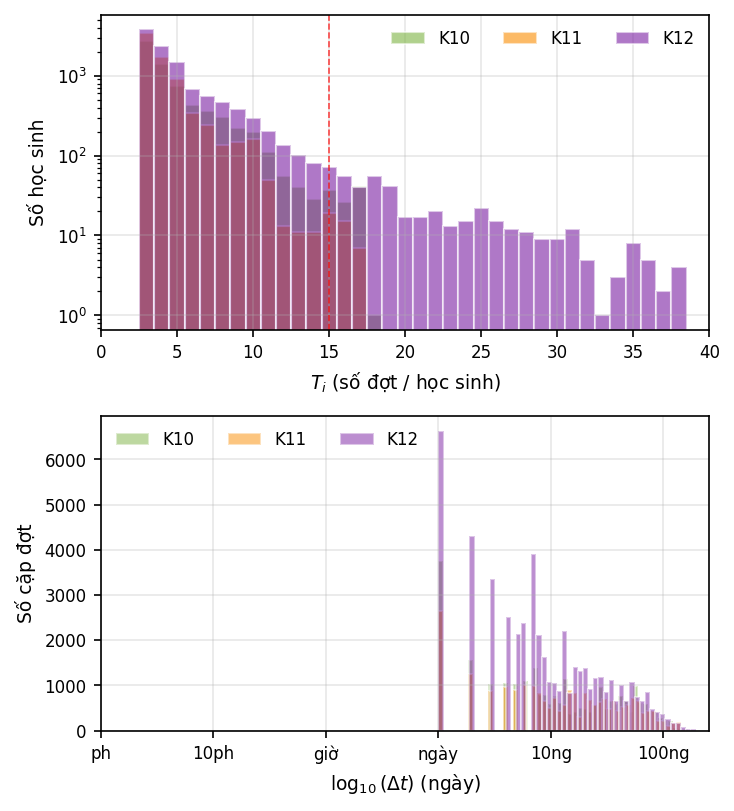
\includegraphics[width=\linewidth]{T_dt_distribution_vertical.png}
  \captionof{figure}{Phân phối $T_i$ (trên) và $\Delta t$ (dưới) theo khối. Đường đứt nét đỏ: ngưỡng $T_i \ge 15$ cho CT-DSEM.}
  \label{fig:Tdt}
\end{minipage}
\end{figure}

\subsubsection{Quy trình phân tích}

Quy trình phân tích gồm bảy bước nối tiếp (Hình~\ref{fig:pipeline}). Nhật ký làm bài trước hết được làm sạch và chuyển sang dạng dài, mỗi dòng là một đáp ứng của một học sinh với một câu hỏi trong một đợt (bước 1). Tính đơn chiều của ngân hàng câu hỏi được kiểm tra bằng phân tích nhân tố khám phá và biểu đồ giá trị riêng (bước 2) trước khi hiệu chuẩn độ khó \(b_j\) bằng mô hình 1PL, riêng cho từng khối (bước 3). Với các \(b_j\) đã cố định, năng lực của học sinh ở từng đợt được chấm bằng EAP, cho cặp \((\hat\theta_{it}, \seit)\) (bước 4). Chuỗi ước lượng này đi vào hai nhánh song song: các mô hình cấu trúc dọc phân tích quỹ đạo ở cấp khối (bước 5), còn bộ làm trơn Kalman hiệu chỉnh quỹ đạo của từng học sinh (bước 6). Kết quả của hai nhánh, cùng ngân hàng câu hỏi đã hiệu chuẩn, được dùng cho hai ứng dụng cảnh báo sớm và gợi ý câu hỏi (bước 7). Bước 1 được viết bằng Python; các bước còn lại dùng R với các gói \texttt{mirt}, \texttt{lavaan}, \texttt{lme4}, \texttt{ctsem} và \texttt{KFAS}.

\begin{figure}[H]
\centering
\resizebox{0.9\linewidth}{!}{%
\begin{tikzpicture}[
  font=\footnotesize,
  every node/.style = {align=center},
  box/.style   = {rectangle, draw, rounded corners=2pt, minimum width=24mm, minimum height=9mm, inner sep=2pt},
  arr/.style   = {-{Latex[length=1.6mm]}, thick},
  dasharr/.style = {-{Latex[length=1.6mm]}, thick, dashed, gray!70},
]
\node[box, fill=gray!12]   (s1) at (0,    0) {(1) Tiền xử lý\\ \scriptsize nhật ký $\to$ dạng dài};
\node[box, fill=blue!8]    (s2) at (3.5,  0) {(2) Kiểm tra đơn chiều\\ \scriptsize EFA, giá trị riêng};
\node[box, fill=blue!8]    (s3) at (7.0,  0) {(3) Hiệu chuẩn 1PL\\ \scriptsize độ khó $b_j$};
\node[box, fill=blue!8]    (s4) at (10.5, 0) {(4) Chấm điểm EAP\\ \scriptsize $\hat\theta_{it},\ \seit$};
\node[box, fill=orange!15] (s5) at (7.2, -1.8) {(5) Mô hình cấu trúc dọc\\ \scriptsize LGCM, LCSM, đa cấp, CT-DSEM};
\node[box, fill=green!15]  (s6) at (11.6,-1.8) {(6) Làm trơn Kalman\\ \scriptsize quỹ đạo từng học sinh};
\node[box, fill=red!12]    (s7) at (9.4, -3.4) {(7) Ứng dụng\\ \scriptsize cảnh báo sớm, gợi ý câu hỏi};
\draw[arr] (s1) -- (s2);
\draw[arr] (s2) -- (s3);
\draw[arr] (s3) -- (s4);
\draw[arr] (s4) -- (s5);
\draw[arr] (s4) -- (s6);
\draw[arr] (s5) -- (s7);
\draw[arr] (s6) -- (s7);
\draw[dasharr] (s3.south) to[bend right=30] (s7.west);
\end{tikzpicture}}
\caption{Quy trình phân tích bảy bước (mũi tên đứt nét: gợi ý câu hỏi dùng ngân hàng câu hỏi đã hiệu chuẩn ở bước 3).}
\label{fig:pipeline}
\end{figure}

% Tuyên bố Đạo đức và bảo mật dữ liệu đã được di chuyển xuống cuối bài
% (gộp cùng Lời cảm ơn + Mã nguồn) theo chuẩn paper quốc tế.

% ============================================================================
% §2.3 Kết quả — 5 bảng + 2 figure key, ~1.8 trang
% ============================================================================

\subsection{Kết quả}
\label{sec:results}

\subsubsection{Kiểm định đơn chiều, độ tin cậy và độ phù hợp các mô hình LSEM}

\textit{Tính đơn chiều} của ngân hàng câu hỏi được đánh giá bằng phân tích nhân tố khám phá (EFA) + biểu đồ giá trị riêng (Hình~\ref{fig:scree}), tương tự bước kiểm tra giả định đơn chiều trước khi chọn mô hình IRT cho đề kiểm tra Toán THPT trong \cite{buhay2026shstat}. Mặc dù tỷ trọng phương sai chung (ECV) chỉ đạt 0{,}56--0{,}68 (chưa đạt ngưỡng nghiêm ngặt 0{,}80 của đơn chiều thuần tuý), tỷ số giá trị riêng \(\lambda_1/\lambda_2 = 2{,}8\)--6{,}0 cho thấy \emph{nhân tố thứ nhất chiếm ưu thế rõ rệt}; điều này biện minh cho việc sử dụng 1PL --- vốn được biết là robust với sai lệch nhẹ khỏi đơn chiều thuần tuý. Khối~12 có ưu thế đơn chiều mạnh nhất (\(\lambda_1/\lambda_2 = 6{,}0\)), phù hợp với việc khối 12 cũng cho ước lượng \(\hat\theta\) tin cậy nhất ở các phân tích phía sau.

\textit{Độ tin cậy} của \(\hat{\theta}\) được tính theo công thức \(\rho = 1 - \overline{\seit^2}/\widehat{\Var}(\hat\theta)\), đạt 0{,}687 / 0{,}746 / 0{,}814 lần lượt cho ba khối. Khối~10 nằm ngay dưới ngưỡng thông thường (\(\rho \ge 0{,}70\)) --- đây là điểm cần lưu ý khi triển khai các ứng dụng ở cấp cá nhân cho khối này. Tất cả sáu mô hình LSEM (LGCM và LCSM cho ba khối) đều đạt \textit{độ phù hợp} tốt với CFI \(> 0{,}99\), RMSEA \(< 0{,}031\) và SRMR \(< 0{,}017\) (Bảng~\ref{tab:rho_fit}).

\begin{figure}[H]
\centering
% --- Bảng 2 (gộp cùng Hình 3 — cùng nói về chất lượng đo lường) ---
\captionof{table}{Độ tin cậy $\rho$ của $\hat\theta$ và chỉ số độ phù hợp của LGCM/LCSM, theo khối.}
\label{tab:rho_fit}
\footnotesize
\begin{tabular}{l rr  rrrrr  rrrrr}
\toprule
 & \multicolumn{2}{c}{\textbf{Đo lường}} & \multicolumn{5}{c}{\textbf{LGCM}} & \multicolumn{5}{c}{\textbf{LCSM}} \\
\cmidrule(lr){2-3}\cmidrule(lr){4-8}\cmidrule(lr){9-13}
\textbf{Khối} & \textbf{$\overline{\seit^2}$} & \textbf{$\rho$} & \textbf{$\chi^2$} & \textbf{df} & \textbf{CFI} & \textbf{RMSEA} & \textbf{SRMR} & \textbf{$\chi^2$} & \textbf{df} & \textbf{CFI} & \textbf{RMSEA} & \textbf{SRMR} \\
\midrule
10 & 0{,}261 & 0{,}687 & 17{,}08 & 5 & 0{,}996 & 0{,}019 & 0{,}011 &  7{,}11 & 2 & 0{,}998 & 0{,}020 & 0{,}008 \\
11 & 0{,}295 & 0{,}746 & 38{,}45 & 5 & 0{,}991 & 0{,}031 & 0{,}017 &  6{,}81 & 2 & 0{,}999 & 0{,}019 & 0{,}007 \\
12 & 0{,}206 & 0{,}814 & 32{,}50 & 5 & 0{,}997 & 0{,}023 & 0{,}011 & 15{,}20 & 2 & 0{,}998 & 0{,}025 & 0{,}010 \\
\bottomrule
\end{tabular}
\par\vspace{4pt}
% --- Hình 3 (Scree) ---
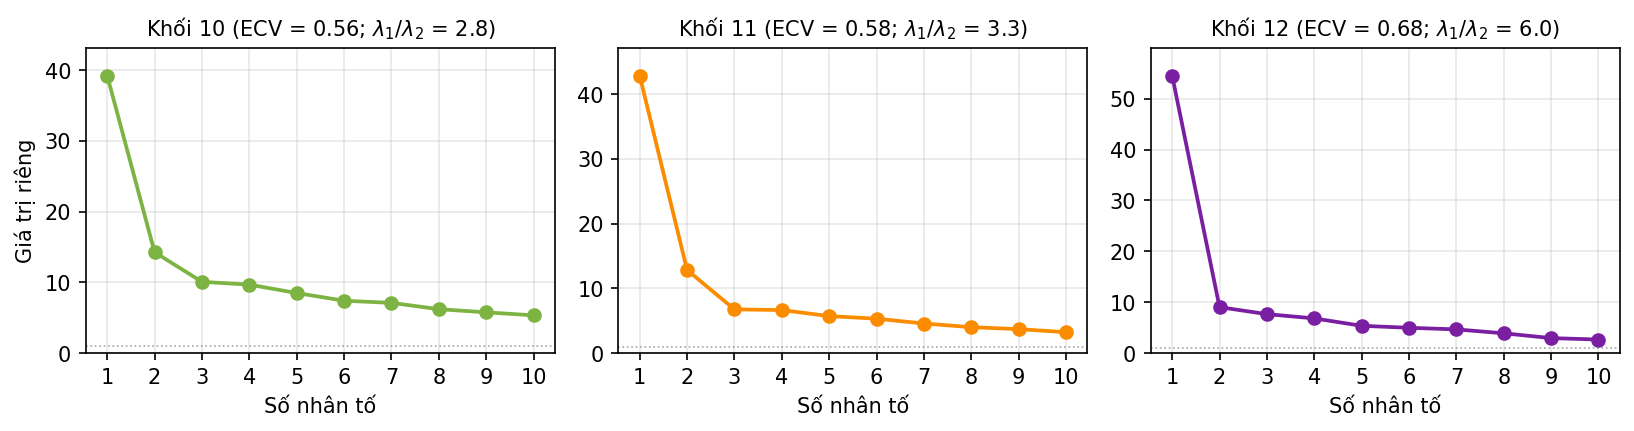
\includegraphics[width=\linewidth]{scree_plots.png}
\captionof{figure}{Biểu đồ giá trị riêng (\emph{scree plot}) theo khối. ECV: tỷ trọng phương sai chung; $\lambda_1/\lambda_2$: tỷ số nhân tố 1 trên nhân tố 2 (càng lớn càng đơn chiều).}
\label{fig:scree}
\end{figure}

\subsubsection{Quỹ đạo tăng trưởng theo khối: từ đuổi kịp đến ổn định}

Hệ số tăng trưởng LGCM dương ở cả ba khối, song độ lớn khác nhau rõ rệt: khối~11 tăng nhanh nhất (\(s = 0{,}028\) logit mỗi đợt, khoảng tin cậy không chứa 0), khối~10 ở mức trung bình (\(s = 0{,}015\)), khối~12 gần như đi ngang (\(s = 0{,}006\)). Hệ số ghép cặp \(\beta\) của LCSM (Hình~\ref{fig:lgcmlcsm}, ô phía trên bên phải) cho thấy một khuôn mẫu thay đổi rất rõ rệt theo khối lớp:
\begin{itemize}
  \item Khối~10: \(\beta = -0{,}069\); khoảng tin cậy 95\% \([-0{,}119,\ -0{,}022]\) \textbf{không chứa 0} --- cơ chế đuổi kịp có ý nghĩa thống kê.
  \item Khối~11: \(\beta = -0{,}043\); khoảng tin cậy 95\% chứa 0 --- xu hướng đuổi kịp đã suy yếu, không còn ý nghĩa thống kê.
  \item Khối~12: \(\beta = +0{,}002\); khoảng tin cậy 95\% chứa 0 và đối xứng quanh 0 --- trạng thái ổn định, không còn ghép cặp.
\end{itemize}

Diễn giải thực tiễn: ở khối~10, một học sinh có \(\theta_{t-1} = -1\) logit (yếu hơn trung bình khối khoảng một độ lệch chuẩn) được kỳ vọng tăng thêm \(|\beta| \cdot 1 \approx 0{,}07\) logit so với học sinh ở mức trung bình ở đợt tiếp theo --- tương đương khoảng 1{,}7\% xác suất trả lời đúng một câu có độ khó trung bình. Hiệu ứng này cộng dồn qua nhiều đợt: sau 5 đợt đánh giá, học sinh yếu được dự đoán đuổi kịp xấp xỉ 0{,}3 logit, tức khoảng 7\% xác suất đúng một câu trung bình so với học sinh khá cùng khối.

\begin{figure}[H]
\centering
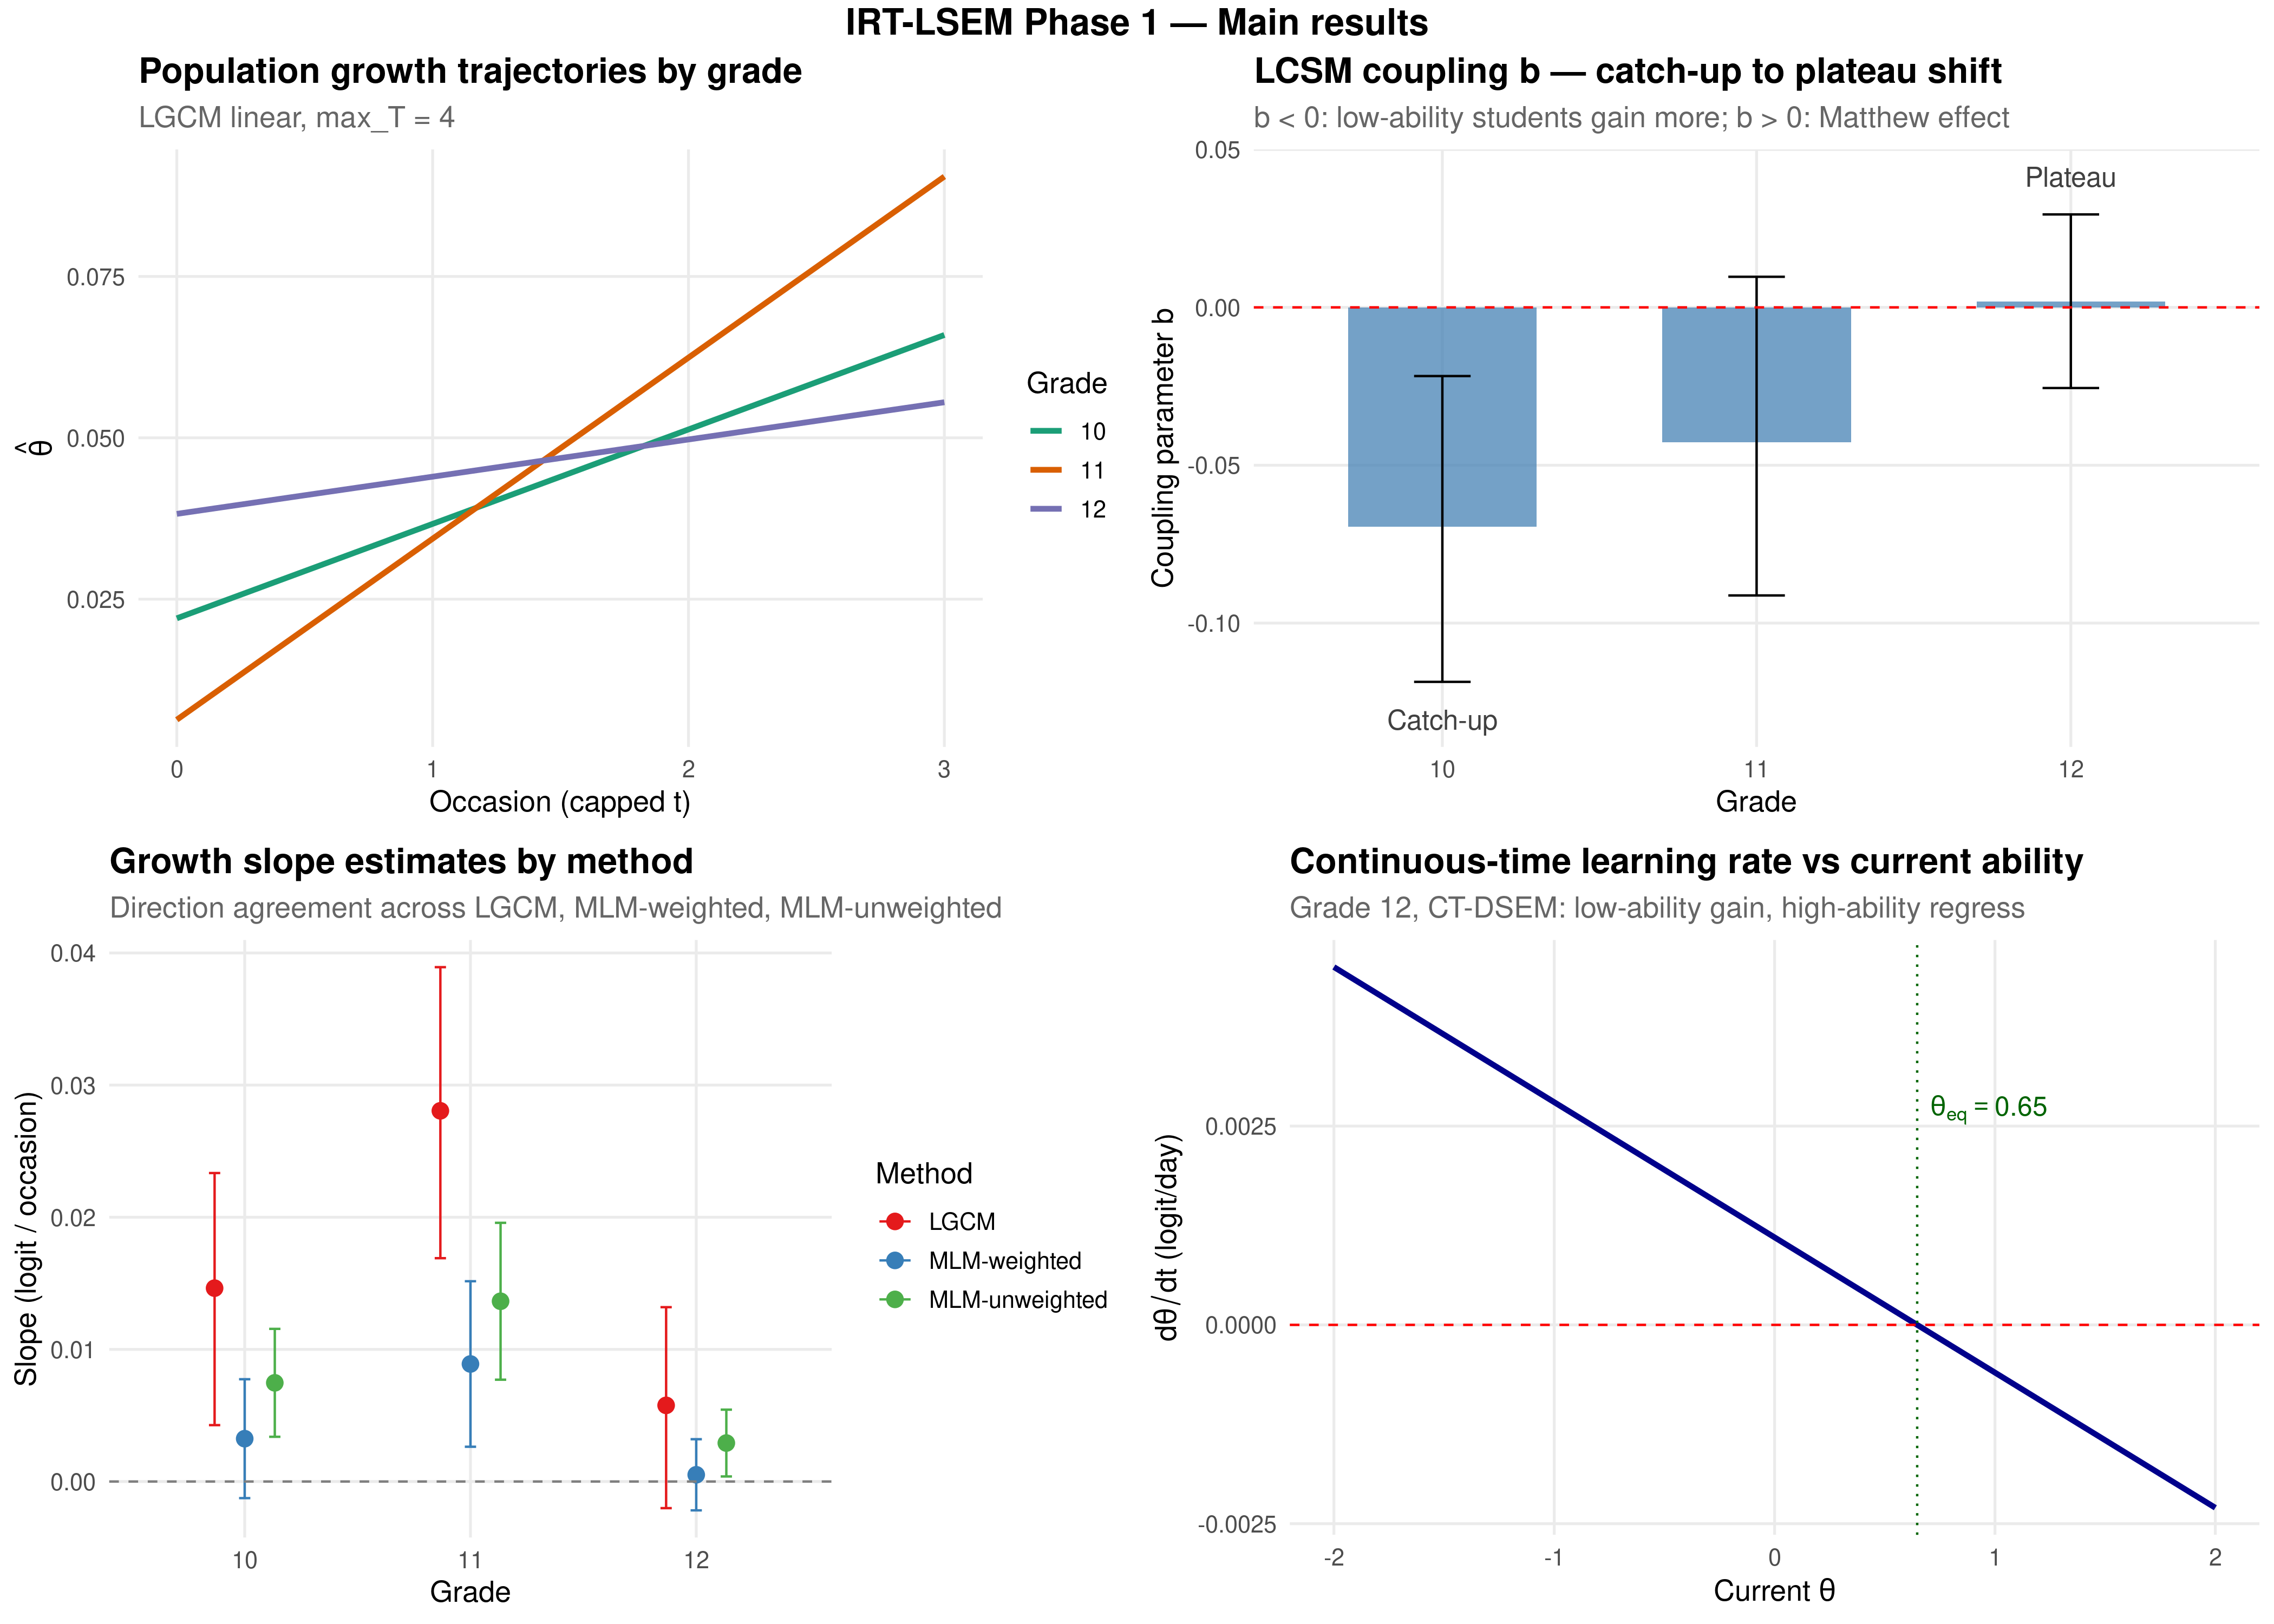
\includegraphics[width=0.95\linewidth]{main_results.png}
\caption{Bốn kết quả chính: quỹ đạo LGCM, hệ số ghép cặp \(\beta\) LCSM, độ dốc đồng dấu từ ba phương pháp, và tốc độ học CT-DSEM ở khối 12 (khối 10/11/12 = xanh lá / cam / tím).}
\label{fig:lgcmlcsm}
\end{figure}

\subsubsection{So sánh thống kê giữa mô hình động và mô hình tĩnh cơ sở}

So sánh AIC/BIC và Kiểm định Tỷ số Hợp lý (Likelihood Ratio Test, LRT) giữa mô hình tĩnh (chỉ có hệ số chặn) và mô hình động (hệ số chặn cộng độ dốc) khẳng định ưu thế áp đảo của mô hình động (Bảng~\ref{tab:lrt}). \(\Delta\)AIC ở mức 82--167 vượt xa ngưỡng thông thường 10 (mức bằng chứng mạnh); giá trị \(p\) của LRT nhỏ hơn \(10^{-19}\) ở cả ba khối và đạt mức \(3 \times 10^{-37}\) ở khối~12.

\begin{table}[H]
\centering\small
\caption{So sánh mô hình tĩnh (chỉ có chặn) với mô hình động (chặn + độ dốc).}
\label{tab:lrt}
\begin{tabular}{lrrrr}
\toprule
\textbf{Khối} & \textbf{$\Delta$AIC} & \textbf{$\Delta$BIC} & \textbf{LRT $\chi^2$ (df=3)} & \textbf{$p$-value} \\
\midrule
10 &  82 &  57 &  87{,}8 & $6{,}5 \times 10^{-19}$ \\
11 &  92 &  67 &  97{,}7 & $4{,}9 \times 10^{-21}$ \\
12 & 167 & 140 & 172{,}9 & $3{,}0 \times 10^{-37}$ \\
\bottomrule
\end{tabular}
\end{table}

\subsubsection{CT-DSEM khối 12: động lực chậm về điểm cân bằng}

Trên tập con khối~12 có \(T_i \ge 15\) (\(N = 460\) học sinh), các tham số của mô hình Ornstein--Uhlenbeck (Bảng~\ref{tab:ctdsem}) cho thấy \(\varphi = -0{,}0017\) (khoảng tin cậy âm, động lực quay về điểm cân bằng), điểm cân bằng dài hạn \(\theta_{\mathrm{eq}} = +0{,}65\) logit (tương ứng \(\approx 66\%\) xác suất trả lời đúng câu trung bình) và bán chu kỳ 408 ngày (vượt một năm học). Tại \(\theta = -1\), tốc độ kỳ vọng đạt \(+0{,}0028\) logit/ngày, tương đương khoảng \(+0{,}25\) logit/học kỳ; tại \(\theta = +1\), tốc độ là \(-0{,}0006\) logit/ngày --- học sinh giỏi có hiện tượng hồi quy về trung bình (\emph{regression to the mean}) nhẹ ngay trong khối~12.

\begin{table}[H]
\centering\small
\caption{Tham số CT-DSEM ở cấp tổng thể (khối 12, $T_i \ge 15$, $N = 460$).}
\label{tab:ctdsem}
\begin{tabular}{lrr}
\toprule
\textbf{Tham số} & \textbf{Ước lượng} & \textbf{CI 95\%} \\
\midrule
$\varphi$ (hệ số trôi)              & $-0{,}0017$ & $[-0{,}0027, -0{,}0010]$ \\
$\mu \varphi$ (hằng số tích phân)   & $+0{,}0011$ & $[+0{,}0006, +0{,}0016]$ \\
$\sigma$ (khuếch tán)               & $0{,}046$   & $[0{,}041, 0{,}053]$ \\
phương sai quan sát $\sigma_\varepsilon^2$ & $0{,}572$ & $[0{,}562, 0{,}582]$ \\
$\theta_{\mathrm{eq}}$              & $+0{,}65$   & --- \\
bán chu kỳ (ngày)                   & 408         & --- \\
\bottomrule
\end{tabular}
\end{table}

\subsubsection{Tác dụng làm trơn của bộ lọc Kalman}

Bộ lọc Kalman cục bộ giúp giảm phương sai sai số đo lường EAP từ 32{,}0\% đến 41{,}2\% mà không cần tăng số câu hỏi khảo sát (Bảng~\ref{tab:ks}, Hình~\ref{fig:kalman}). Phương sai trạng thái ước lượng được \(\hat q_g\) phản ánh biến thiên \emph{thực} của năng lực giữa các đợt đánh giá: khối~11 dao động lớn nhất (\(\sqrt{q} \approx 0{,}86\) logit), gợi ý rằng đây là giai đoạn năng lực biến động mạnh nhất trong ba khối THPT --- nguyên nhân cụ thể (cường độ luyện tập, áp lực thi cử, hay đặc trưng nội dung môn học) cần các nghiên cứu mở rộng để xác định.

\begin{figure}[H]
\centering
\begin{minipage}[c]{0.50\linewidth}
  \centering\footnotesize
  \captionof{table}{Hiệu quả của bộ lọc Kalman: $\overline{\seit}$ giảm và $\hat q_g$ theo khối.}
  \label{tab:ks}
  \resizebox{\linewidth}{!}{%
  \begin{tabular}{lrrrr}
  \toprule
  \textbf{Khối} & \textbf{$\overline{\seit}$ thô} & \textbf{$\overline{\seit}$ làm trơn} & \textbf{Giảm \%} & \textbf{$\hat q_g$} \\
  \midrule
  10 & 0{,}499 & 0{,}387 & 41{,}2 & 0{,}444 \\
  11 & 0{,}527 & 0{,}433 & 34{,}3 & 0{,}734 \\
  12 & 0{,}442 & 0{,}369 & 32{,}0 & 0{,}620 \\
  \bottomrule
  \end{tabular}%
  }
\end{minipage}\hfill
\begin{minipage}[c]{0.48\linewidth}
  \centering
  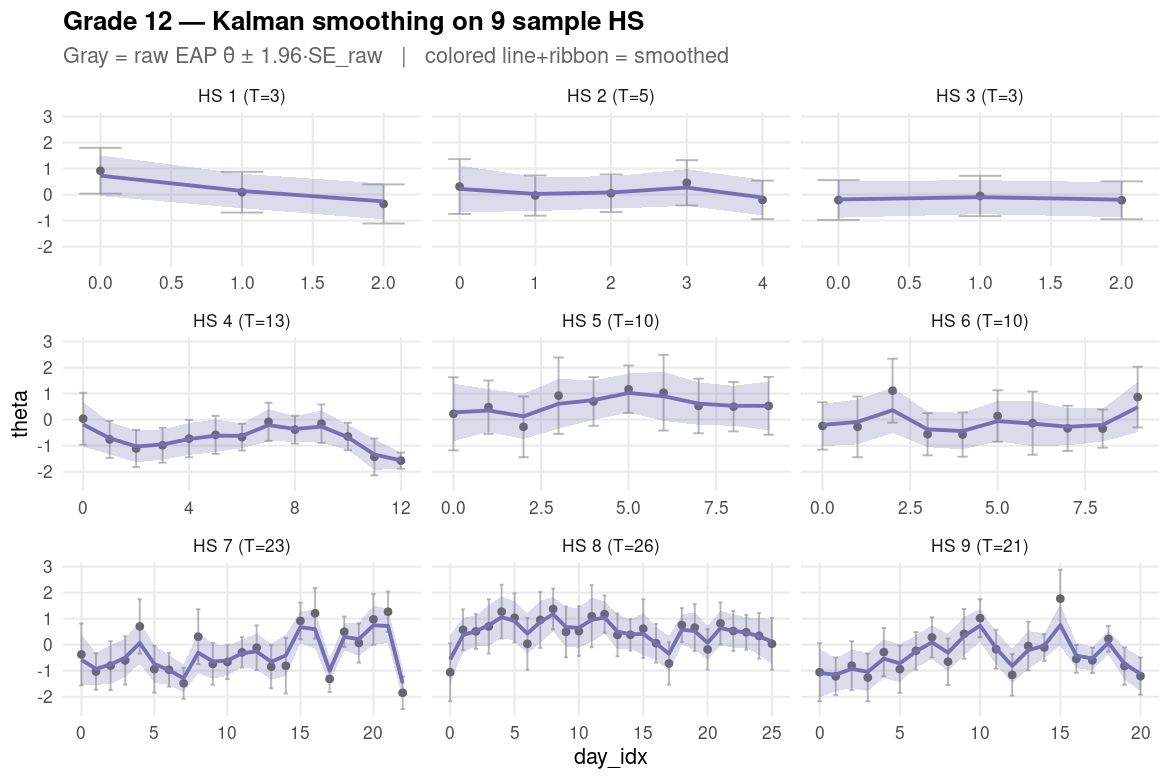
\includegraphics[width=\linewidth]{kalman_overlay_g12.png}
  \captionof{figure}{Chín học sinh khối 12 (ẩn danh): chấm xám = $\hat\theta$ EAP thô, đường liền = quỹ đạo Kalman.}
  \label{fig:kalman}
\end{minipage}
\end{figure}

\subsubsection{Ứng dụng: cảnh báo sớm và gợi ý câu hỏi}

Trên quỹ đạo đã làm trơn, tổng tỷ lệ học sinh bị đánh dấu tăng dần từ khối 10 lên khối 12 (từ 14{,}4\% lên 22{,}3\%; Bảng~\ref{tab:warning}). Nhóm học sinh thoả mãn đồng thời cả hai tiêu chí (tốc độ tăng trưởng thấp và xuất hiện bước giảm đột ngột) duy trì ở mức 3{,}5--5{,}7\% qua ba khối --- đây là tập học sinh cần được giáo viên ưu tiên rà soát thủ công.

Đối với bài toán gợi ý câu hỏi (B7b), 100\% các câu được khuyến nghị có \(|b - \hat\theta_{i,T}| < 0{,}5\) (150 hàng minh hoạ, ứng với 10 học sinh đại diện $\times$ 5 câu $\times$ 3 khối). Tỷ lệ này chủ yếu phản ánh \emph{mật độ cao của ngân hàng câu hỏi} ở vùng độ khó trung bình (Hình~\ref{fig:diff_dist}) chứ không phải đặc thù riêng của thuật toán; đóng góp của bài nằm ở chỗ gợi ý được căn cứ trên quỹ đạo đã làm trơn (phản ánh xu thế gần đây của học sinh) thay vì dựa trên một ước lượng \(\hat\theta\) tĩnh duy nhất.

\begin{figure}[H]
\centering
% --- Bảng 6 ---
\captionof{table}{Số học sinh được cảnh báo sớm theo khối. Cột ``Cả hai'': học sinh thoả mãn đồng thời cả hai tiêu chí (tốc độ tăng trưởng thấp và bước giảm đột ngột).}
\label{tab:warning}
\small
\begin{tabular}{lrrr rrr}
\toprule
\textbf{Khối} & \textbf{$N$ đủ điều kiện} & \textbf{Tổng đánh dấu} & \textbf{\%} & \textbf{Chỉ độ dốc} & \textbf{Chỉ bước giảm} & \textbf{Cả hai} \\
\midrule
10 &  6{.}285 &   905 & 14{,}4 & 411 &   276 & 218 \\
11 &  6{.}740 & 1{.}357 & 20{,}1 & 293 &   683 & 381 \\
12 & 10{.}440 & 2{.}325 & 22{,}3 & 557 & 1{.}281 & 487 \\
\bottomrule
\end{tabular}
\par\vspace{4pt}
% --- Hình 6 (Phân phối độ khó) — dùng layout 3-panel ngang ---
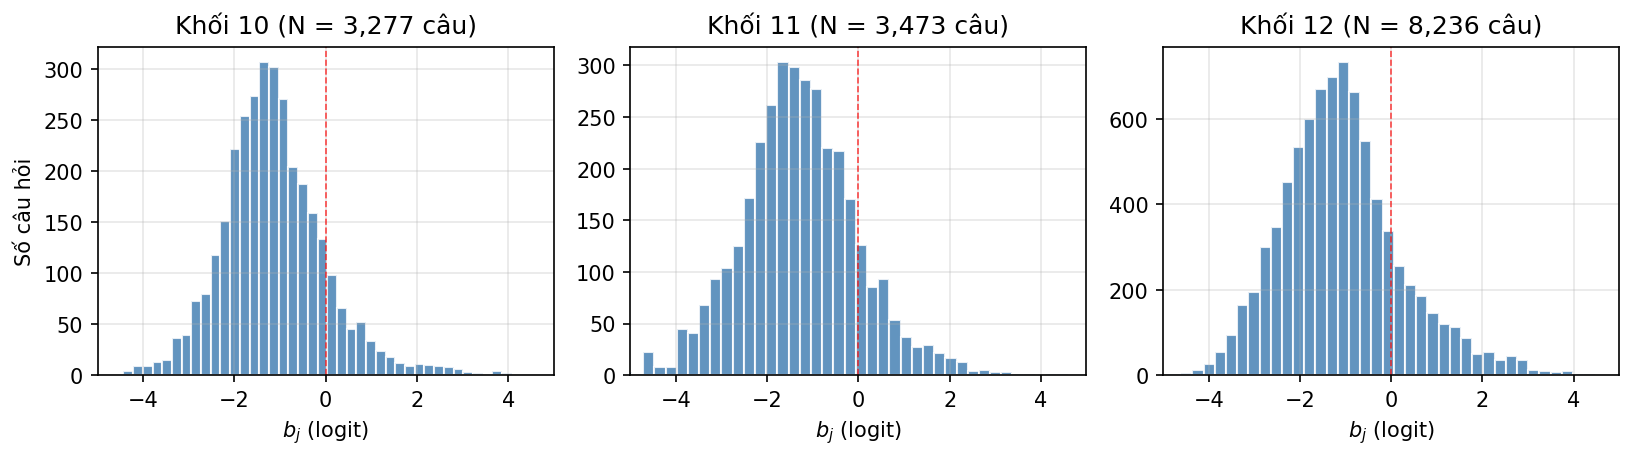
\includegraphics[width=0.95\linewidth]{difficulty_dist_all_grades.png}
\captionof{figure}{Phân phối độ khó $b_j$ theo khối (đường đứt nét đỏ: $b = 0$).}
\label{fig:diff_dist}
\end{figure}

% ============================================================================
% §2.4 Thảo luận — văn phong tiếng Việt học thuật.
% ============================================================================

\subsection{Thảo luận}
\label{sec:discussion}

\textbf{Diễn giải chính:} Sự nhất quán giữa hệ số ghép cặp \(\beta\) của LCSM (Hình~\ref{fig:lgcmlcsm}) và các tham số CT-DSEM của khối~12 (Bảng~\ref{tab:ctdsem}) cho thấy một quỹ đạo phát triển năng lực gồm hai pha: pha đuổi kịp ở khối~10 --- nơi học sinh có năng lực thấp được kéo về mặt bằng chung của lớp; và pha ổn định ở khối~12 --- nơi nhóm học sinh đã hội tụ về một điểm cân bằng tương đối cao (\(\theta_{\mathrm{eq}} \approx +0{,}65\)) với động lực rất chậm (bán chu kỳ vượt một năm học). Hệ quả thực tiễn: các can thiệp ngắn hạn khó dịch chuyển đáng kể giá trị \(\theta\); muốn tạo thay đổi rõ rệt về năng lực, cần các can thiệp đủ mạnh và kéo dài --- đây là gợi ý quan trọng cho phụ huynh và giáo viên khi lập kế hoạch học tập.

\textbf{Đối chiếu giữa các phương pháp:} Hệ số tăng trưởng ước lượng bằng LGCM (theo phương pháp FIML) và bằng lmer (theo phương pháp REML) đồng dấu (dương) ở cả ba khối, tuy nhiên chênh lệch tuyệt đối \(|s_{\mathrm{LGCM}} - s_{\mathrm{lmer}}|\) lớn hơn 0{,}005 ở mọi khối (Bảng~\ref{tab:convergent}). Khác biệt này xuất phát từ cách xử lý dữ liệu thiếu: FIML khai thác toàn bộ thông tin sẵn có thông qua giả định tăng trưởng tuyến tính, trong khi REML chỉ sử dụng các quan sát đầy đủ. Các kết luận định tính của nghiên cứu --- mô hình động vượt mô hình tĩnh và cơ chế đuổi kịp chuyển dần sang trạng thái ổn định theo khối --- giữ được tính bền vững; tuy nhiên độ lớn tuyệt đối của các tham số cần được hiểu trong giới hạn của thuật toán ước lượng được chọn.

\begin{table}[H]
\centering\small
\caption{Đối chiếu độ dốc $s$ ước lượng bằng LGCM (FIML) và lmer (REML).}
\label{tab:convergent}
\begin{tabular}{lrrr}
\toprule
\textbf{Khối} & \textbf{$s_{\mathrm{LGCM}}$} & \textbf{$s_{\mathrm{lmer}}$} & \textbf{$|$chênh lệch$|$} \\
\midrule
10 & 0{,}0146 & 0{,}0032 & 0{,}0114 \\
11 & 0{,}0281 & 0{,}0089 & 0{,}0192 \\
12 & 0{,}0058 & 0{,}0005 & 0{,}0053 \\
\bottomrule
\end{tabular}
\end{table}

\textbf{Giới hạn nghiên cứu:} (1) \emph{Cấu hình mẫu và tính khái quát hoá} --- Trung vị \(T_{\mathrm{median}} = 4\text{--}5\) đợt là ngắn so với chuẩn vàng LSEM bậc hai (\(T \ge 6\)) và RI-CLPM đa biến tiềm ẩn; mẫu là người dùng OLM tự chọn nền tảng học trực tuyến, không đại diện ngẫu nhiên cho tổng thể học sinh THPT; hiệu lực cấu trúc của \(\hat\theta\) so với các thang đo truyền thống (điểm trường, thi quốc gia) chưa được đối chiếu. (2) \emph{Hồi quy về trung bình do sai số đo} --- Hệ số \(\beta\) của LCSM được ước lượng từ \(\hat\theta\) EAP vốn có sai số đo và bị co rút về phân phối tiên nghiệm; do đó một phần \(\beta < 0\) ở khối 10 có thể phản ánh hồi quy về trung bình do độ tin cậy hữu hạn (\(\rho = 0{,}687\)) thay vì cơ chế đuổi kịp thực chất --- khuôn mẫu \(\rho\) thấp đi kèm \(|\beta|\) lớn (khối 10) và \(\rho\) cao đi kèm \(\beta \approx 0\) (khối 12) phù hợp với cả hai cách diễn giải. Việc tách biệt đòi hỏi mô phỏng hiệu chỉnh hoặc mô hình hoá sai số đo ở tầng tiềm ẩn. (3) \emph{Tính tương thích của thang đo qua thời gian} --- Năng lực ước lượng \(\hat\theta\) ở các đợt được chấm với cùng tiên nghiệm \(N(0,1)\), chưa thực hiện căn chỉnh thang đo dọc (\emph{vertical scaling}) hay kiểm định trôi tham số (DIF) theo thời gian; việc neo trung bình quần thể tại mỗi đợt có thể thu hẹp ước lượng tăng trưởng ở cấp tổng thể. (4) \emph{Bộ làm trơn hồi cứu so với bộ ước lượng trực tuyến} --- Kalman trong bài là bộ làm trơn (\emph{smoother}) dùng quan sát tương lai chứ không phải bộ lọc đệ quy thuần trực tuyến; mục tiêu ước lượng thời gian thực sau mỗi đáp ứng mới (gắn với phát biểu bài toán) chưa được hiện thực hoá. Mở rộng cho quan sát phi tuyến (1PL/2PL) qua Suy diễn Biến phân đã có thiết kế nhưng chưa có mã chạy thực tế. (5) \emph{Cỡ mẫu lớn và các giả định đo lường chặt} --- Với \(N\) rất lớn, \(\Delta\)AIC và \(p\)-value LRT phản ánh chủ yếu cỡ mẫu; độ dốc thực 0{,}006--0{,}028 logit mỗi đợt cho thấy việc ``bác bỏ giả định tĩnh'' chủ yếu mang ý nghĩa thống kê, còn độ lớn tín hiệu động vẫn khiêm tốn. Ba giả định cần kiểm chứng: bất biến đo lường giữa bài luyện tập (nỗ lực thấp) và kiểm tra (nỗ lực cao); mô hình 1PL bỏ qua tham số đoán ngẫu nhiên \(c_j\); và giả định đơn chiều cho môn Toán đa chủ đề (Đại số, Hình học, Giải tích). (6) \emph{Ứng dụng chưa được kiểm chứng hiệu quả thực tế} --- B7a chưa đối chiếu độ chính xác và độ thu hồi (\emph{precision} và \emph{recall}) với kết quả học tập về sau; tỷ lệ 100\% câu khuyến nghị trong ngưỡng \(\delta = 0{,}5\) ở B7b chủ yếu phản ánh mật độ ngân hàng câu hỏi chứ không phải chất lượng của thuật toán. Ngoài ra, mô hình trạng thái Kalman dạng bước ngẫu nhiên (\emph{random walk}) mâu thuẫn với cơ chế hồi quy về trung bình (\emph{mean-reverting}) mà CT-DSEM phát hiện ở khối 12, và bộ làm trơn có thể làm mờ các bước giảm đột ngột mà cảnh báo sớm cần phát hiện --- hiện tượng làm trơn quá mức (\emph{over-smoothing}) cần được cân nhắc khi triển khai. Bài toán đánh giá hiệu quả giảng dạy và bộ dữ liệu thứ hai (đánh giá định kỳ STEM ở trường phổ thông) đều đòi hỏi mở rộng dữ liệu (thông tin lớp/giáo viên hoặc hợp tác trường), nằm ngoài phạm vi bài báo này.


% ============================================================================
% §3 Kết luận — văn phong hedged, consistent với §2.4 limitations (RTM,
% effect size khiêm tốn, smoother hồi cứu).
% ============================================================================

\section{Kết luận}
\label{sec:conclusion}

Bài báo đề xuất và kiểm chứng một khung tích hợp IRT--LSEM kèm bộ lọc Kalman trên bộ dữ liệu OLM Toán THPT quy mô lớn (24{.}213 học sinh, 122{.}957 lượt đánh giá thuộc năm học 2024--2025). Ba phát hiện chính:

(1) Mô hình động vượt mô hình tĩnh cơ sở \emph{về mặt thống kê} với \(\Delta\)AIC = 82--167 và \(p\)-value LRT \(\le 10^{-19}\); tuy nhiên độ lớn các tham số tăng trưởng thực (độ dốc 0{,}006--0{,}028 logit mỗi đợt) còn khiêm tốn --- tín hiệu động tồn tại nhưng cần đánh giá ý nghĩa thực tiễn trong từng bối cảnh ứng dụng cụ thể.

(2) Một xu thế giảm dần của hệ số ghép cặp \(\beta\) theo khối lớp được quan sát (khối 10 \(\beta = -0{,}069\) với khoảng tin cậy không chứa 0; khối 12 \(\beta \approx 0\)), nhất quán với điểm cân bằng dài hạn \(\theta_{\mathrm{eq}} = +0{,}65\) và bán chu kỳ 408 ngày của CT-DSEM. Cần thận trọng khi diễn giải kết quả này như cơ chế đuổi kịp thực chất, vì một phần có thể phản ánh hồi quy về trung bình do sai số đo lường hữu hạn (xem giới hạn 2 ở Mục~\ref{sec:discussion}); việc phân tách hai nguồn này là một hướng kiểm chứng quan trọng cho các nghiên cứu mở rộng.

(3) Bộ lọc Kalman làm trơn hồi cứu (\emph{smoother}) giảm 32--41\% phương sai sai số đo lường EAP trong cùng quy trình phân tích mà không cần tăng số câu hỏi khảo sát --- đây là cải thiện kỹ thuật rõ rệt và độc lập với hai phát hiện trên về cấu trúc.

Các hướng nghiên cứu mở rộng được đề xuất gồm: (a) triển khai mã chạy thực tế của Suy diễn Biến phân cho 1PL nhằm hiện thực hoá ước lượng đệ quy thuần trực tuyến (mục tiêu thời gian thực) và so sánh với Kalman trên cùng tập dữ liệu; (b) căn chỉnh thang đo dọc qua năm học (vertical scaling) bằng cách sử dụng các đề ôn 2025--2026 làm câu hỏi neo (anchor items); (c) tích hợp siêu dữ liệu lớp học và giáo viên để mở rộng phân tích sang bài toán đánh giá hiệu quả giảng dạy dựa trên tốc độ tăng trưởng năng lực; (d) tách biệt cơ chế đuổi kịp thực chất khỏi hồi quy về trung bình do sai số đo bằng mô phỏng hiệu chỉnh hoặc mô hình hoá sai số đo ở tầng tiềm ẩn; (e) mở rộng phân tích sang biến tiềm ẩn thứ hai (mức độ tương tác, thời gian học) để khôi phục tính xác định của mô hình RI-CLPM.

% ============================================================================
% Cụm tuyên bố cuối bài: Lời cảm ơn + Đạo đức + Mã nguồn — đều ngắn gọn (10pt).
% ============================================================================

\section*{Lời cảm ơn}
\label{sec:ack}

{\fontsize{10}{12}\selectfont
Tác giả cảm ơn PGS.\,TS.\,Phạm Thọ Hoàn (người hướng dẫn chính) và Công ty Cổ phần Khoa học và Công nghệ Giáo dục OLM đã hỗ trợ nghiên cứu này.
\par}

\section*{Đạo đức và dữ liệu}

{\fontsize{10}{12}\selectfont
\noindent Dữ liệu do OLM cung cấp theo điều khoản dịch vụ, phục vụ mục đích nghiên cứu khoa học giáo dục phi thương mại. Định danh học sinh đã được hash hoá trước khi phân tích, đảm bảo không thể nhận diện ngược cá nhân. Bài báo chỉ công bố các kết quả tổng hợp; dữ liệu chi tiết của từng học sinh được tác giả chia sẻ riêng cho mục đích tái lập nghiên cứu khi có yêu cầu chính đáng từ các nhà nghiên cứu khác.
\par}

\section*{Khai báo sử dụng trí tuệ nhân tạo}

{\fontsize{10}{12}\selectfont
\noindent Trong quá trình thực hiện nghiên cứu, tác giả sử dụng mô hình ngôn ngữ lớn Claude (Anthropic), thông qua công cụ Claude Code, vào hai việc: (i) hỗ trợ viết và gỡ lỗi mã nguồn phân tích bằng R và Python của quy trình B0--B7; (ii) hỗ trợ tìm kiếm và tóm tắt tài liệu liên quan. Toàn bộ mã nguồn do AI hỗ trợ đã được tác giả rà soát và chạy lại trên dữ liệu; mọi tài liệu trích dẫn đã được tác giả đối chiếu với bản gốc. Tác giả chịu hoàn toàn trách nhiệm về nội dung, số liệu và kết luận của bài báo.
\par}

\section*{Mã nguồn}

{\fontsize{10}{12}\selectfont
\noindent Mã nguồn quy trình phân tích và các kết quả tổng hợp có tại \url{https://github.com/dtnntd/irt-lsem}.
\par}


% ============================================================================
% TÀI LIỆU THAM KHẢO — 11pt, xếp theo thứ tự xuất hiện trong bài (style/hnue.bst):
%   "Tác giả, năm. Tên bài. Tạp chí (in nghiêng). Vol. xx, Số. xx, tr. xx-xy."
% ============================================================================

\renewcommand{\refname}{\fontsize{11}{13}\selectfont TÀI LIỆU THAM KHẢO}
{\fontsize{11}{13}\selectfont
\bibliographystyle{style/hnue}
\bibliography{refs/references}
\par}


% ============================================================================
% ABSTRACT tiếng Anh — cuối bài, sau Tài liệu tham khảo (theo mẫu bài tiếng Việt):
%   - "ABSTRACT" 11pt; tên bài tiếng Anh chữ thường, in đậm, 11pt.
%   - Tác giả 12pt; đơn vị in nghiêng 11pt; tóm tắt 11pt.
% ============================================================================

\begin{english}
\vspace{4pt}

\begin{center}
{\fontsize{11}{13}\bfseries\selectfont ABSTRACT}
\end{center}
\vspace{-6pt}
\begin{center}
{\fontsize{11}{13}\bfseries\selectfont
Dynamic estimation of student ability based on Item Response Theory (IRT) and Longitudinal Structural Equation Modeling (LSEM)}
\end{center}
\vspace{-6pt}
\begin{center}
{\fontsize{12}{14}\selectfont
Nguyen Tien Dat\textsuperscript{1}}
\end{center}
\vspace{-6pt}
\begin{center}
{\fontsize{11}{13}\itshape\selectfont
\textsuperscript{1}Faculty of Information Technology, School of Mathematics and Information Technology,\\
Hanoi National University of Education, Hanoi, Vietnam}
\end{center}

{\fontsize{11}{13}\selectfont
\noindent Item Response Theory (IRT) systems deployed at scale, including Vietnam's OLM platform, typically assume a static student ability~\(\theta\), yet large-scale online learning produces densely longitudinal data that contradicts this assumption. We construct and validate an integrated IRT--LSEM framework for estimating dynamic ability~\(\theta_{it}\) on real OLM Mathematics data covering 24{,}213 high-school students and 122{,}957 assessment occasions across grades 10--12. The framework couples a 1PL measurement layer (EAP scoring) with four structural layers (LGCM, LCSM, multilevel growth, continuous-time DSEM) and a Kalman smoother that exploits EAP standard errors as time-varying observation noise. The dynamic model beats the static-Rasch baseline by \(\Delta\)AIC = 82--167 (LRT \(p \le 10^{-19}\)); LCSM reveals catch-up at grade 10 (\(\beta = -0.069\), CI excludes 0) shifting to plateau at grade 12; Kalman cuts mean EAP error variance by 32--41\% with no extra items.\par
\noindent\textbf{\textit{Keywords:}} Item Response Theory, longitudinal structural equation modeling, Kalman smoothing, dynamic ability estimation, educational data mining.
\par}
\end{english}


\end{document}
